% !TEX root = ../maturaarbeit.tex
\chapter{Implementation Details}\label{chap:in_practice}
In this chapter I will apply Reinforcement Learning to a simplified simulation of soccer. I will go over the environment specification, the agent implementation, training results and what was required to get there.

\section{Frameworks and Tools}\label{sec:ip:tools}
In this section I will briefly go over the main tools I used for my work and provide reasons for why I opted to use them.
\subsection{Python}\label{subsec:ip:tools:python}
%Machine Learning Libraries
I used Python as the main language to write my agent code in mainly because of all the data science and machine learning libraries present for it. Tools like NumPy \cite{noauthor_numpy_nodate}, TensorFlow all provide highly performant and parallel backends for data storage, manipulation and vectorized operations. This also nullifies the relatively bad performance of python, very few operations are actually performed by it.
\nolinebreak
%Low iteration times
Another major plus for python is the low iteration time when developing for it. Because it is interpreted rather than compiled there is no waiting time for code to compile and live python environments like IPython \cite{noauthor_ipython_nodate} and Jupyter Notebook \cite{noauthor_jupyter_nodate} enable excellent testing.
\nolinebreak
%Modularity
Last but not least there is the excellent standard library of python. It makes asynchronous programming, file handling efficient storage through Deques and general boiler plate operations easy.

\subsection{TensorFlow 2}\label{subsec:ip:tools:tensorflow}
%what
TensorFlow is a Machine Learning API \cite{noauthor_tensorflow_nodate}. I use it due to my prior familiarity with it and its broad set of features. It is widely adopted and enables parallel execution of vectorized operation on GPUs through CUDA and cuDNN. Furthermore it also provides tools for FIFO-queues and data visualization through TensorBoard. TensorFlow 2.X allows for the use of compiled computational graphs, as well in place "eager" execution of operations. It has provisions for automatic differentiation and through its Keras \cite{chollet2015keras} module makes building Artificial Neural Networks simple.

\subsection{Unity ML-Agents}\label{subsec:ip:tools:ml_agents}
%what
I use the Unity ML-Agents toolkit \cite{juliani2020unity} \cite{noauthor_unity-technologiesml-agents_2020} for my environment implementation. It provides example environments under the Apache 2.0 license, I use a modified version of one of them. 
\nolinebreak
%why
I opted to use this toolkit because of my prior knowledge with the Unity game engine it is based in, its flexibility in creating and modifying environments, it's visual appeal, the possibility of easily implementing human input in order to play against trained agents (where such play applies) and the high quality environments which come prepackaged.


\section{The Environment}\label{sec:ip:environment}
\begin{figure}[H]
    \centering
    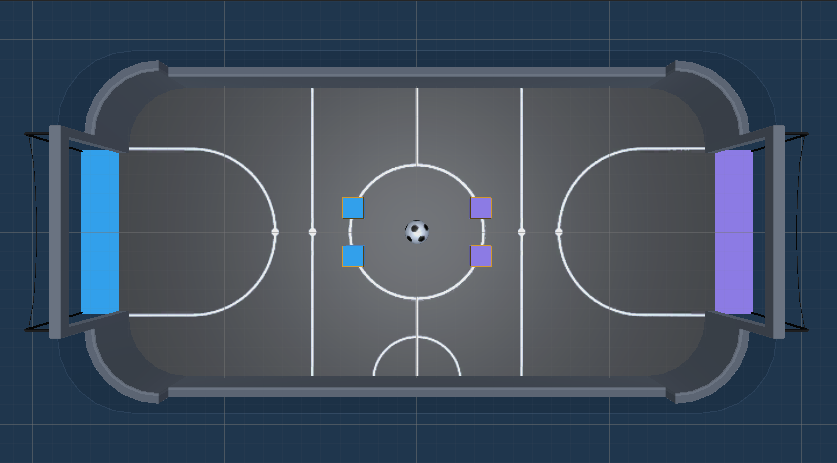
\includegraphics[width=0.7\linewidth]{figures/soccer_field.png}
    \caption{A screenshot of the soccer field taken from the Unity editor}
    \label{fig:soccer_field}
\end{figure}

\noindent
%Overview with image
Here I will lay out the workings of the environment I opted to use, explain the integration with with python, and go over some of the code crucial to its function. This section describes the baseline  modified "Soccer" environment. "Soccer" is the name used in the ML-Agents toolkit. I work with variations on it in \ref{sec:tr:variations}, they all depend on this baseline. The environment I use to train the agent is a simplified version of a game of soccer. 

\subsection{Suitability for my Work}\label{subsec:ip:environment:suitabilty}
At the beginning of this thesis I was faced with the decision whether I should use a preexisting environment or create my own. I opted to make use of an already existing one since this was more in line with my lead question, which asks how an agent is trained. I chose this specific environment because it presents a decent balance between complexity, likelyhood of successful training, intrigue and extensibilty. High extensibilty lowers the barrier to training agents on variations of it, thereby having a measure of how adaptable my methodology it is. Further after the modifications I made to the environment it now also offers continuous control to the agent, this presents an interesting challenge, relevant to real world task, where input is seldom binary.

\subsection{Specifics of Operation}\label{subsec:ip:environment:implementation}
The baseline environment is in function mostly identical to the "Soccer" example environment provided by the Unity ML-Agents toolkit. Here I will go over it's sequence of operation, it's specification, and state all the changes I made to it in order to make it suit my work better. The game of soccer takes place on a bounded field and has four players, distributed across two teams. Each Player is its own Agent, they all act on the same policy and all produce trajectories for it's training. Thereby the policy is trained in play against itself. 

\newpage

\subsubsection{Observations}\label{subsubsec:ip:environment:impl:observations}

\begin{figure}[H]
    \centering
    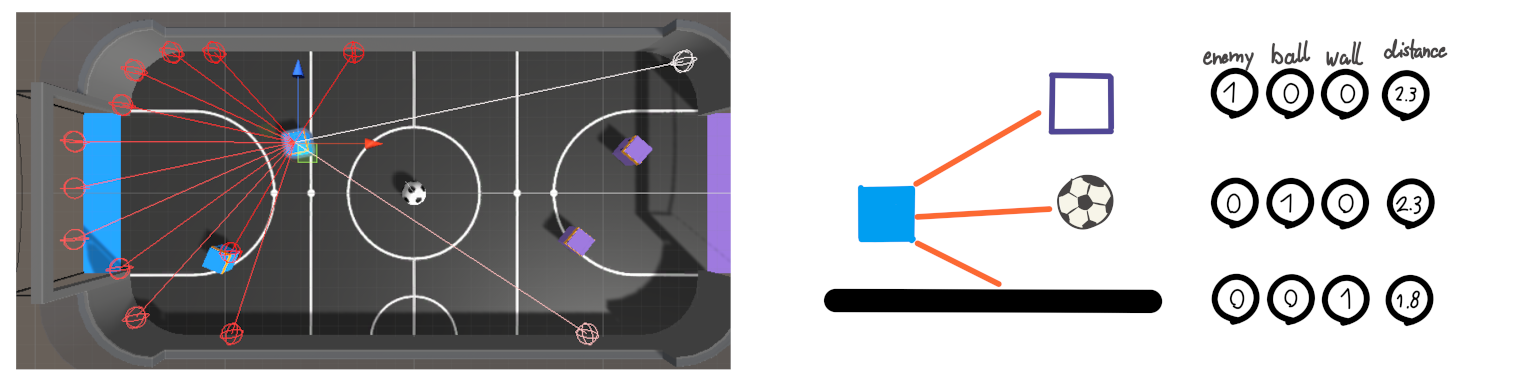
\includegraphics[width=1\linewidth]{figures/ray_sensor.png}
    \caption{Caption}
    \label{fig:ray_sensor}
\end{figure}
\noindent
The "Soccer" example environment uses "Ray Perception Sensors" to create an observation for the agent. A ray perception sensor works by casting a number of rays spread out through a predefined field of view. Along each of these rays a sphere is slid, starting at the agents position and stopping on collision with an object. Each ray contains information about the distance to the object it hit, and its type. The types are predefined, in the case of "Soccer" they are "wall", "enemy", "teammate", "team goal", "enemy goal" and "ball". To the agent a vector is then passed, consisting of the distance to the object the ray struck, as well as its one-hot encoded type. The above figure illustrates how one-hot encoding works and how the observation vectors looks for each ray. The observation vectors are then concatenated to form one single vector, this is then used as the input layer of my policy network. One-hot encoding is commonly used in machine learning where a type information needs to be passed as input, this way separate trainable weights are present for each category. The episode ends if either a goal is score, or a maximum of $600$ time steps pass.

\subsubsection{Episode Start}\label{subsubsec:ip:environment:impl:start}
One subtle but important change I made to the "Soccer" environment is that I randomize agent position and rotation at the beginning of each episode. 

\begin{lstlisting}[basicstyle=\footnotesize]
public override void OnEpisodeBegin() {
    timePenalty = 0;
    m_BallTouch = m_ResetParams.GetWithDefault("ball_touch", 1f);
    transform.rotation = Quaternion.Euler(0, (Convert.ToSingle(random.NextDouble()) - 0.5f) * m_RandomSpawnRotationOffset, 0);
    transform.position = m_Transform + new Vector3((Convert.ToSingle(random.NextDouble()) - 0.5f) * m_RandomSpawnPositionOffset, 0, (Convert.ToSingle(random.NextDouble()) - 0.5f) * m_RandomSpawnPositionOffset);
    agentRb.velocity = Vector3.zero;
    agentRb.angularVelocity = Vector3.zero;
    SetResetParameters();
}
\end{lstlisting}
I made this change because without it during initial testing, agents would come to learn to simply move forward and all clash in to one another. The ball would then fly off in some direction, often scoring a goal for one of the teams. Because of this no real gameplay would arise. While the merits of this change are debatable, i opted for it. This chose was made from personal preference and in the interest gameplay intrigue.

\subsubsection{Actions}\label{subsubsec:ip:environment:impl:actions}
The environment takes continuous action input from the agent. This was not the case in the example environment provided. Three single precision floating point values are expected, they represent forward, lateral, and rotational movement respectively. This is the \code{C\#} code I use to move the agent:

\begin{lstlisting}[basicstyle=\footnotesize]
public void MoveAgent(ActionSegment<float> act) {
    m_KickPower = 0f;

    float longitudinalAxis = Convert.ToSingle(System.Math.Tanh(act[0])) * m_ForwardSpeed;
    float lateralAxis = Convert.ToSingle(System.Math.Tanh(act[1])) * m_LateralSpeed;
    float rotationalAxis = Convert.ToSingle(System.Math.Tanh(act[2]));

    Transform transformTMP;
    (transformTMP = transform).Rotate(transform.up, rotationalAxis * 6.5f);
    agentRb.AddForce(
        (transformTMP.forward * longitudinalAxis +
         transformTMP.right * lateralAxis)
        * m_SoccerSettings.agentRunSpeed,
        ForceMode.VelocityChange);
}
\end{lstlisting}
\noindent
As visible here, I use the scaled arctangent of the action values received. This is to prevent unexpected behaviour which might result when the values the agent selects are too large. The scaling values for forward and lateral speed are the same as the ones used in the "Soccer" example environment. They are \code{m\_LateralSpeed \= 0.3f;} and \code{m\_ForwardSpeed \= 1.0f;}. The \code{agentRunSpeed} is \code{2.0f}.

%Continuous Action Space
%tanh to bind 
\subsubsection{Rewards}\label{subsubsec:ip:environment:impl:rewards}
In the baseline environment I use the rewards provided by the ML-Agents toolkit. The only rewards given to the agent over the course of the episode are on collision with the ball, in which case a reward of \code{0.2} is given, and the end of the episode. This reward is \code{1.0 + timePenalty} if the episode terminated because the agents team managed to score a goal, if the episode ended in a draw or the agent's team lost it is \code{-1.0}. The \code{timePenalty} is accumulated at every time step according to \code{timePenalty -= m_Existential;}, with \code{m_Existential} being the inverse of the maximum episode length. If there was no time penalty it might me more advantageous for the agents to only repeatedly hit the ball instead of scoring goals.
%perform same action for 10 steps
%quit after n steps
%random agent heurisitc 
%Some Code Snippets 
\subsection{Communication with Policy in Python}\label{subsec:ip:environment:communication_python}
One of the reasons the ML-Agents toolkit is particularly appealing is because it allows for extensive control of the environment in Python. The toolkit provides a Python side API with the \code{mlagents} and \code{mlagents_envs} modules. The figure below, taken from \cite[p. 12]{juliani2020unity}, illustrates this interface.

\begin{figure}[H]
    \centering
    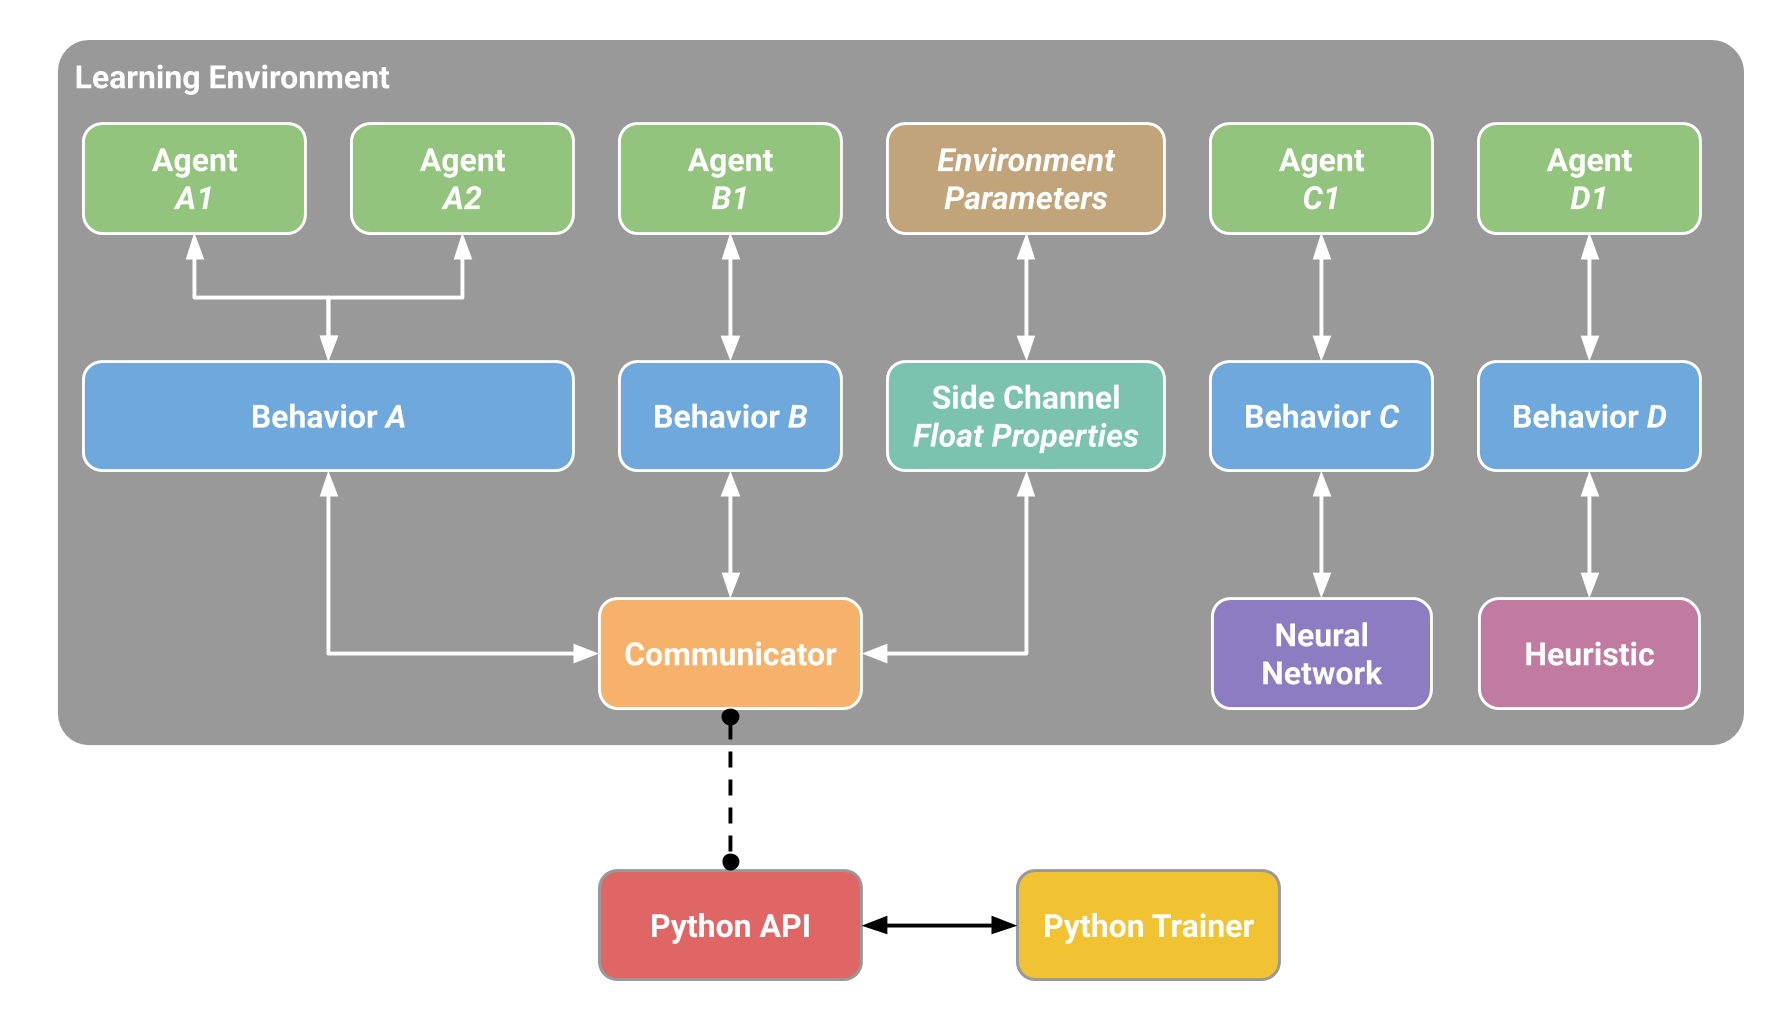
\includegraphics[width=0.75\linewidth]{figures/ml_agents_python_communicator.png}
    \caption{Illustration of communication between Unity and Python}
    \label{fig:python_communicator}
\end{figure}

\noindent
Through the Python API it is possible to train multiple agents, with possibly differing behaviours (formally, each of these behaviours represent a different environment because the observations and actions, as well as the underlying environment functions differ from those of other behaviours, they are effectively different MDPs, see section \ref{sec:MDP}), and even to have yet other agents running on inference (acting on policies which are not being updated, here "Neural Network") or heuristics. This allows for tremendous flexibility not only in training but also enabled me to more fully consider my lead question which also pertains to observation, action and reward design. On the Python side of the ML-Agents training framework there exists, the \code{UnityEnvironment} class. Instantiating it launches, and creates an interface with, a Unity executable \cite[p. 13]{juliani2020unity}. From an instance of \code{UnityEnvironment} information about the observation and action type and size can be obtained. During training and evaluation observations, actions, stepping of the environment, and restarting episodes are all handled through this class's members.

\section{Agent Implementation}\label{sec:ip:agent_implementation}
In this section I will go over the agent implementation in Python. This encompasses the architecture of the Neural Network and the components necessary for training and evaluating an agent.

\subsection{Agent Policy}\label{subsec:ip:agent:network}
In \ref{subsec:ip:environment:implementation} I explained the layout of the observation provided by the environment. With it and knowledge of what type of actions the environment expects, the policy network can be constructed. Both of these can be obtained through an instance of the \code{UnityEnvironment} class, \code{env} in the code below:

\begin{lstlisting}[basicstyle=\footnotesize]
for name, spec in env.behavior_specs.items():
    action_shape = spec.action_shape
    observation_shape = np.sum(np.concatenate(spec.observation_shapes))
\end{lstlisting}

\noindent
I concatenate and sum across \code{spec.observation_shapes} because unity separates ray cast observations up based on internal structure. This separation is useless to me, this is why I undo it here. \code{env.behaviour_specs} is a mapping from behaviour names, to their implementation details. To obtain an action for a continuous environment I sample from a normal distribution following the theory outlined in \ref{subsec:pg:continuous}. For the mean $\mu$ I make use of an MLP \ref{sec:neural_networks}, for the standard deviation $\sigma$ I implement a single trainable parameter for each action. Both are obtained from a Keras model created by by the function found in appendix \ref{appendix:code:network}, following the TensorFlow Keras functional API \cite{noauthor_tensorflow_nodate}\cite{chollet2015keras}. I will first cover the Network used to obtain the mean, then go over how the full normal distribution and action is obtained.

\subsubsection{Neural Network Used for the Mean}\label{subsubsec:ip:agent:policy:mean}
The number of neurons in the last layer before the mean output is the smallest power of two larger than the number of continuous actions and at least $32$. The number of neurons in the input layer is the largest power of two smaller than the dimension of the input vector, and at least four times the number of neurons in the last layer before the output. In between the layers decay in size, each subsequent layer is smaller than the previous by a factor of two. The resulting network looks as follows for the baseline soccer environment:

\begin{figure}[H]
    \centering
    
\includegraphics[width=0.5\linewidth]{figures/placeholder.png}
    \caption{Network Structure}
    \label{fig:network_repr}
\end{figure}

\noindent
This structure provided stable results during initial testing. By creating a comparatively smooth reduction in unit count across layers, each neuron has to encode a limited amount of information. I did not first step up the layer size because for the task at hand, an initial layer size of $256$ seemed sufficient. The last layer does also not have an activation function, and its bias is initialized to be zero. This leads to untrained initial mean values centered on zero. During initial testing this lead to higher stability and likelyhood of convergence on a performant policy. This is also suggested in \citepg{335}. For baseline training I use rectified linear units \cite[pg. 189]{Goodfellow-et-al-2016}, neurons with $\max(0, x)$ as the activation. Neurons using this go by the name of "ReLU", Rectified Linear Units. I initialize the weights in this network using the initialization proposed in \cite[p. 251]{glorot_understanding_2010}, where weights are sampled from $U\left[ -\frac{1}{\sqrt{n}}, \frac{1}{\sqrt{n}} \right]$ with $n$ being the number of units in the previous layer, I will refer to this method of initialization as "glorot uniform". Since I could not find any conclusive evidence on what the best activation and method of initialization are, these choices are mostly arbitrary, and reflect the default options of the Keras API. I cover alternatives in \ref{sec:tr:param_tweaking}.

\subsubsection{Single Trainable Variables for Standard Deviation}\label{subsubsec:ip:agent:policy:std}
Creating input independent trainable variables can be a bit tricky in Keras, especially in conjunction with it's model saving system. However, it is possible by subclassing \code{tensorflow.keras.Layer}. I created such a sub classed custom Keras layer, the respective code follows. In it \code{tensorflow} is aliased by \code{tf}:

\begin{lstlisting}[basicstyle=\footnotesize]
class IndependentTrainableVarLayer(tf.keras.layers.Layer):
    def __init__(self, name: str, initializer: K.initializers.Initializer, shape):
        self.shape = shape
        self.initializer = initializer
        super().__init__()

    def build(self, shape):
        self.x = self.add_weight(name=self.name, shape=self.shape, initializer=self.initializer)

    def call(self, _, **kwargs):
        return tf.identity(self.x)

    def compute_output_shape(self, input_shape):
        return input_shape[0], 1

    def get_config(self):
        return {'shape': self.shape, 'initializer': self.initializer}   
\end{lstlisting}

\noindent
It does not matter what \code{call()} is called on, but Keras expects an input. Further, simply returning self.x is also not possible due to Tensorflows internals. This class is used in the full model code found in \ref{appendix:code:network}.
\subsubsection{Obtaining an Action}
The graph for the combined model for for the mean and standard deviation returned by \ref{appendix:code:network} looks as follows:

\begin{figure}[H]
    \centering
    
\includegraphics[width=0.5\linewidth]{figures/placeholder.png}
    \caption{Structure of baseline Keras model}
    \label{fig:full_model_graph}
\end{figure}

\noindent
From this model the means and standard deviations for a given observation can the be obtained by simply calling it on said observation, an action can then be constructed with \code{tensorflow.random.normal()}. It's first argument is the output shape of the actions, its second are the respective means, and its last the standard deviations. A Keras model expects the first dimension of the input tensor to correspond to a batch of inputs. The resulting output will correspond to the batched input, the model is applied to each item of the input batch. This is convenient since \code{UnityEnvironment} provides the observation for each of its agents in one tensor where the first dimension corresponds to the agents. Thereby the actions for every agent following a particular policy can be obtained with the following method:

\begin{lstlisting}[basicstyle=\footnotesize]
@tf.function
def _get_actions(self, obs) -> tf.Tensor:
    mu, sig = self.policy_network(obs)
    actions: tf.Tensor = tf.random.normal(mu.shape, mu, sig)
    return actions
\end{lstlisting}

\noindent
The \code{@tf.function} decorator results in TensorFlow creating a compilable computational graph in its backend. This enables highly parallel execution. However, in a \code{@tf.function} decorated function, the number of legal operations is limited to the ones supported by TensorFlow. it also returns a \code{tf.Tensor}. For the data contained to be usable for \code{UnityEnvironment}, it needs to be converted to a \code{numpy.ndarray}. This can be done by calling its \code{tf.Tensor.numpy()} method, and caching its return value. 

\subsection{Parameter Update}\label{subsec:ip:agent:training_func}
Having the policy as a Keras model provides for highly efficient training and using Tensorflows inbuilt tools for gradient descent. One of those tools is Tensorflows automatic differentiation. In TensorFlow 2.X this feature is recommended to be accessed through the \code{tensorflow.GradientTape()} context manager. Using it the parameter update presented in \ref{subsec:pg:continuous} can be performed using the following mehtod:

\begin{lstlisting}[basicstyle=\footnotesize]
@tf.function
def _policy_train_step(self, states, actions, returns):
    with tf.GradientTape() as tape:
        mu, sig = self.policy_network(states)
        pdf_value = tf.cast(tf.exp(-0.5 * ((actions - mu) / sig) ** 2), tf.float32) * \(1 / (sig * tf.sqrt(tau)))
        log_probabilities = tf.math.log(pdf_value + 1e-5)
        loss_pi = - returns * log_probabilities
        grads_pi = tape.gradient(loss_pi, self.policy_network.trainable_variables)
    grads_pi = [tf.clip_by_norm(g, self.clip_gradients) for g in grads_pi]
    self.policy_optimizer.apply_gradients(zip(grads_pi, self.policy_network.trainable_variables))
\end{lstlisting}

\noindent
Recall the gradient used in the reinforce update:

\begin{equation*}
    G_t \nabla \ln{\pi(A_t | S_t, \theta_t)}
\end{equation*}

First the mean, here \code{mu}, and the standard deviation of the probability distributions are sampled from the policy network for all observations, here \code{states}. Based on these the probability density can then be obtained for the cached action sampled from the normal distributions during an episode. This corresponds to $\pi(A_t | S_t, \theta_t)$. Next the natural log is applied. Finally, the loss, the expression with respect to which the gradient is derived, is \code{loss_pi}. The returns are computed from the rewards through vectorized operations, the function I use for this is to be found in \ref{appendix:code:returns}. The gradients \code{grads_pi} can be obtained using the alias for the context manager \code{tape}. It is noteworthy that all operations here are element wise. The negative of \code{returns * log_probabilities} is used because gradient ascent, is simply gradient descent performed along the negative gradients. The gradients are clipped to prevent unstable updates when they are overly large. The \code{policy_optimizer} is an implementation of Adam (see \ref{subsec:gd:adam}). This works because for the optimization step only the gradients need to be known. Lastly, in \citepg{328} $\theta$ is updated for every timestep in envery episode sampled from environment interaction. However, since $\nabla J(\theta)$ is the expectation of the gradient above, updating with the average of a batch of samples of this gradient is going to yield a better approximation of $\nabla J(\theta)$, Keras' implementation of Adam does exactly this. 

\subsection{Caching Experience and Batched Training}\label{subsec:ip:agent:archive}
Because of restrictions in the speed in which environment interaction is possible, having only a single agent interact with the environment would quickly become a bottleneck for training time. The base "Soccer" environment provided by unity, is laid out for training $32$ agents simultaneously. This has the consequence that the policy cannot be trained after every episode without throwing out all other trajectories, or changing policy mid episode. To deal with this I use two buffer systems. One, encompassed by the \code{Trajectory} class, stores observations, actions, and rewards of an episode. Once the episode terminates, its returns are computed with the method found in \ref{appendix:code:returns}, and the data is fed to a central dataset. The following preprocessing is then applied to the dataset:

\begin{lstlisting}[basicstyle=\footnotesize]
def train(self, states: tf.Tensor, actions: tf.Tensor, returns: tf.Tensor, measurer: Measurer = None):
    dataset_length = states.shape[0]
    indices = np.arange(dataset_length)
    np.random.shuffle(indices)
    for batch in range(dataset_length // self.batch_size):
        batch_indices = indices[batch * self.batch_size: (batch + 1) * self.batch_size]
        self._policy_train_step(
            tf.gather(states, batch_indices),
            tf.gather(actions, batch_indices),
            tf.gather(returns, batch_indices))
\end{lstlisting}

\noindent
This randomizes the order of the environment interaction samples, and breaks the training process up in to batches. This is not an issue, because the rewards are computed beforehand. The randomization is used to break temporal corelation between samples in a batch, thereby including a broader range of states in it. The rational behind this was that a broader range of states and thereby transitions should lead to a better approximation of $\nabla J(\theta)$. Using Adam each batch correlates to a timestep during optimization. Batch size is one of the parameters explored in \ref{sec:tr:param_tweaking}.

\section{End-to-End Training and Evaluation}\label{sec:ip:training_testing}

\subsection{Code Structure}\label{subsec:ip:tt:class_structure}
Here I will briefly go over the code structure I used. The figure below serves to illustrate it:

\begin{figure}[H]
    \centering
    
\includegraphics[width=0.7\linewidth]{figures/placeholder.png}
    \caption{Code structure used in training}
    \label{fig:code_structure}
\end{figure}

\noindent
The Keras model used for policy approximation is wrapped by a subclass of \code{BasePolicyModel}. As such it implements methods for training based on archived training data, saving the Keras model, and providing actions sampled from the policy. Implementations of \code{Agent} hold this model wrapper, as well as an instance of \code{ BaseTrainingBuffer}, and a dictionary, mapping a \code{Trajectory} to all agents following a conceptual Unity behaviour, which an \code{Agent} corresponds to. The main training loop communicates with \code{Agent} and itself acts as an interface between Unity and the Behaviour specific training code. 


\subsection{The Training Loop}\label{subsec:ip:tt:training_loop}
The code below shows the main loop I use to train agents. This loop generalizes for any number of behaviours, for all of which \code{Agent}s are instantiated dynamically at run time based on parameters. However in the case of the baseline "Soccer" environment, there only is a single behaviour, and thereby agent. \code{agents} is a mapping from Unity's behaviour names to \code{Agent} objects.
\begin{lstlisting}[basicstyle=\footnotesize]
for iteration in range(ParameterData.iterations):
    t_step = 0
    while not all(agent.archive.full for agent in agents.values()):
        for name, agent in agents.items():
            decision_steps, terminal_steps = env.get_steps(name)
            actions = agent.get_actions(np.concatenate(decision_steps.obs, 1))
            env.set_actions(name, actions)
            agent.handle_decision_steps(decision_steps, actions)
            agent.handle_terminal_steps(terminal_steps, ParameterData.discount_factor)
        env.step()
        t_step += 1
        
    for name, agent in agents.items():
        agent.train()
        measures = agent.measurer.finalize_and_collect(name)
        current_time = time.time()
        with writer.as_default():
            for key, value in measures.items():
                if value.shape[0] > 1: tf.summary.histogram(key, value, iteration)
                else: tf.summary.scalar(key, value[0], iteration)
            tf.summary.flush()
        agent.save(ParameterData.model_save_dir + f'{start_time}/{current_time}/')
    env.reset()
\end{lstlisting}
\noindent
The training is performed for a number of iterations preset by a parameter. During each iteration the agents interact with the environment until a sufficient number of samples are accumulated. At each timestep, which here is refering to the synchronized time steps with Unity, decision steps and terminal steps are obtained from Unity. \code{agents} is a mapping from Unity's behaviour names to \code{Agent} objects. \code{decision_steps} is of the type \code{DecisionSteps} and contains the rewards for the previous step, and observations based on which Unity expects actions.
\code{terminal_steps} is of type \code{TerminalSteps} but oposed to decision steps it only contains the rewards for the last timestep in an episode. \code{Agent.handle_decision_steps} and \code{Agent.handle_terminal_steps} both handle training data buffering operations. Once all agents have gathered a sufficient amount of training data, their \code{train()} methods are called and performance as well as stability metrics are collected and logged.

\subsection{Training Variables}\label{subsec:ip:tt:params}
Throughout my work I have introduced many Variables. Below I Provide a short table of the ones used in the baseline environment, where they are used, and their their baseline value. \\
\begin{tabular}{ |p{4cm}||p{3cm}|p{3cm}|p{3cm}|  }
 \hline
 \multicolumn{4}{|c|}{Training Parameters} \\
 \hline
 Parameter & Symbol & Value & Used in Section\\
 \hline
 discount factor & $\gamma$ & 0.99 & \ref{subsec:goals}\\
 samples per iteration &  & $524288 = 2^19$ & \ref{subsec:ip:agent:archive}\\
 batch size &  & $16384 = 2^{14}$ &  \ref{subsec:ip:agent:archive}\\
 learning rate (lr) & $\alpha$ & 0.0003 & \ref{gd:what_is_it}\\
 clipping threshold &  & 10 & \ref{subsec:ip:agent:training_func}\\
 1\textsuperscript{st} momentum decay & $\rho_1$ & 0.9 & \ref{subsec:gd:adam}\\
 2\textsuperscript{nd} momentum decay & $\rho_2$ & 0.999 & \ref{subsec:gd:adam}\\
 activation function &  & ReLU & \ref{subsec:ip:agent:network}\\
 initialization method &  & glorot uniform & \ref{subsec:ip:agent:network}\\
 
 \hline
\end{tabular}

\subsection{Evaluation}\label{subsec:ip:tt:eval} 
To evaluate agent performance during training the metric I use is the average return obtained at each time step. However this brings some limitations when comparing to agents using different parameters because fundamentally, agents are performing self play during training. Since the data of both sides is logged, an increase in agent performance is necessarily also also an increase in it's opponents performance. To account for this I am going to choose parameters based on relative performance. Following the example in \cite{juliani2020unity}, I am going to implement an Elo rating. This is the rating system most famously used in chess. The Elo rating of a player $A$ is updated after a game has been played against $B$ by first calculated the expected score according to:

\begin{equation*}
    E_A = \frac{1}{1+10^{\frac{\left(R_B-R_A\right)}{400}}}
\end{equation*}
\noindent
which can be interpreted as the expected probability of $A$ winning. Then, $A$'s Elo rating $R_A$ can be updated:

\begin{equation*}
    R'_A = R_A + k(S_A-E_A)
\end{equation*}
\noindent
Where $k$ is a constant that determines the weight of each game, in my working i am going to use 4. $S_A$ is the actual score which must also be a valid probability in my case 0 for a loss, 1 for a victory, and 0.5 if the episode terminates because the maximum number of time steps were reached. The number 400 is an arbitrary scaling factor, I follow the example of chess in using it. When evaluating each agent starts out with a score of 1000, then that score is adjusted by playing 1000 games against agents trained on every other permutation of a particular parameter.
\noindent
\\ During training I additionally monitor episode length and the $\mu$ and $\sigma$ values of the normal distribution for continuous actions. This gives me some insight in to training process. In addition to this I log the parameters used in training using TensorBoard, TensorFlow's inbuilt logging system. TensorBoard can host a local server which can the be accessed through a client web GUI:

\begin{figure}[H]
    \centering
    
\includegraphics[width=0.6\linewidth]{figures/placeholder.png}
    \caption{TensorBoard}
    \label{fig:tensorboard}
\end{figure}



